\section{Desenvolvimento}

\subsection{Projeto}
%TODO explicar a finalidade deste projeto
Com a finalidade de oferecer uma referência de desenvolvimento de aplicações
Bluetooth no contexto da Internet das Coisas, foi feito um projeto baseado em
microcontroladores que implementa (\ldots) %TODO

O projeto desenvolvido foi o de uma estação de monitoramento de variáveis
ambientais, que tem como funcionalidade principal a realização de leituras
periódicas de sensores com a transmissão sem fio das variáveis medidas
utilizando o bluetooth low energy. Estes dados, quando recebidos por um scanner
bluetooth, são enviados para a internet.

Para tal, dividiu-se as tarefas em três sistemas diferentes, como mostra a
figura \ref{fig:project_overview}:
a estação de medidas, responsável pela coleta e transmissão das medididas através do
bluetooth, o gateway BLE-Internet, responsável por captar os dados no ar e
enviá-los para a internet, e a infraestrutura online, que recebe a informação e
a armazena on-line.

\begin{center}
	\centering 
	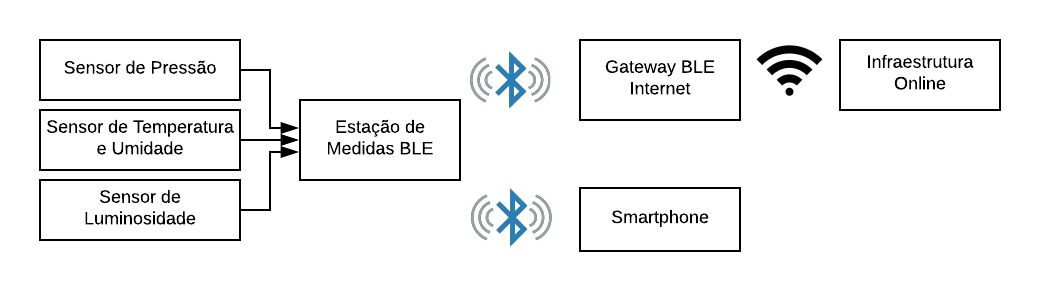
\includegraphics[width=0.5\linewidth]{project_overview.jpg}
	\captionof{figure}{Esquemático dos sistemas presentes no projeto}
	\label{fig:project_overview}
\end{center} 

%TODO justificar as variáveis medidas e os critérios de seleção dos sensores,
% incluindo a disponibilidade de breakout boards

Os sensores escolhidos para o projeto são:
\begin{itemize}
  \item BMP180: Sensor de pressão
  \item TSL2561: Sensor de luminosidade
  \item HTU21D: Sensor de temperatura e umidade
\end{itemize}

Todos os sensores especificados são digitais e possuem características low
power. Além disso, o meio de acesso é o barramento I2C para todos os casos, fato
que auxiliou o desenvolvimento do projeto devido a interface compartilhada entre
todos os dispositivos.

\subparagraph{BMP180} O sensor BMP180, presente no placa da figura
\ref{fig:bmp180breakout} é um sensor de pressão desenvolvido, produzido e vendido pela Bosch. É capaz de
operar com tensões de 1.8V a 3.6V,consumindo uma corrente de 0.1$\mu A$ a 4$\mu
A$ nas temperaturas de $25\,^{\circ}{\rm C}$ e $85\,^{\circ}{\rm C}$ respectivamente. 
Durante a conversão dos valores de pressão, a corrente de pico varia entre 650$\mu A$ a 1000$\mu A$, e durante a operação a $25\,^{\circ}{\rm C}$ com frequência de amostragem de 1Hz, a
corrente consumida fica entre 3$\mu A$ e 32$\mu A$ dependendo da resolução do
configurada. \cite{BMP180Datasheet}

\begin{center}
	\centering 
	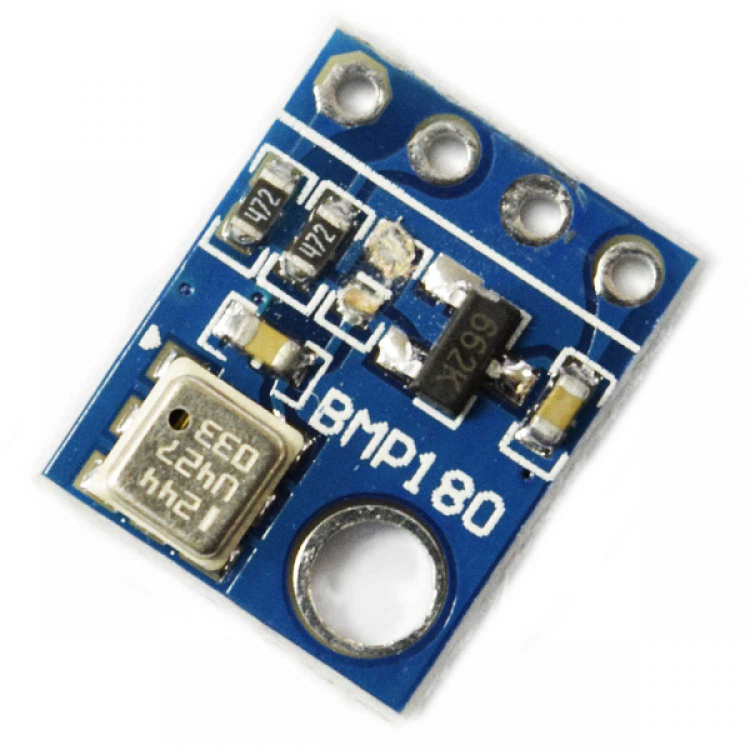
\includegraphics[width=0.5\linewidth]{BMP180.png}
	\captionof{figure}{Módulo de Desenvolvimento para o sensor BMP180}
	\label{fig:bmp180breakout}
\end{center} 


Considerando o tempo máximo de conversão para cada resolução,
estima-se que a frequência de amostragem máxima para este sensor fica entre
222.22Hz(low power mode) e 13Hz(Advanced res. mode). O range de medidas do
sensor é de 30kPa a 110kPa. \cite{BMP180Datasheet}


\subparagraph{TSL2561} O sensor TSL2561, presente na placa da figura
\ref{fig:tsl2561breakout}, é um sensor de luminosidade produzido pela empresa
ams AG que combina um fotodiodo que responde numa larga faixa espectral
(visível e infravermelho) e um fotodiodo que responde somente a faixa
infravermelha do espectro. O sensor possui comunicação I2C que permite a
configuração, leitura e envio de comandos.

\begin{center}
	\centering 
	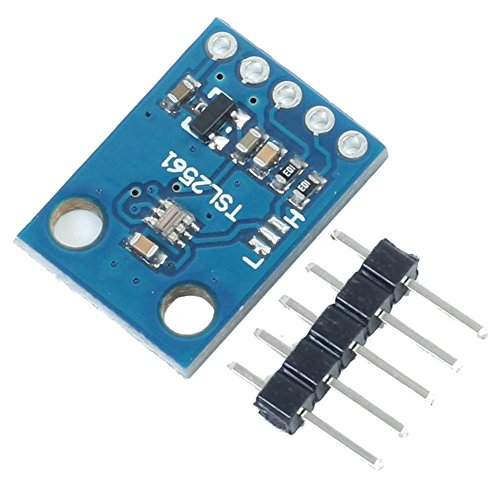
\includegraphics[width=0.4\linewidth]{TSL2561.jpg}
	\captionof{figure}{Módulo de Desenvolvimento para o sensor TSL2561}
	\label{fig:tsl2561breakout}
\end{center} 

Os valores lidos pelo sensor são convertidos para
iluminância em Lux através de uma equalção empírica fornecida pelo fabricante
que busca se aproximar da resposta do olho humano. A característica de possuir
dois fotodiodos permite com que o sensor trabalhe em regiões em que há uma
incidência alta de luz infravermelha, pois com um fotodiodo dedicado ao
infravermelho é possível medir e descontar a influência da luz infravermelha na
medida de luminosidade.\cite{TSL2561Datasheet}

A tensão de alimentação é de até 3.8V. Durante os períodos de conversão de
luminosidade, o consumo de corrente varia entre 0.24mA e 0.6mA. Já no modo
power down, o consumo de corrente varia entre 3.2$\mu A$ e 15$\mu A$. Possui
uma resolução de 16 bits na saída do ADC que realiza as conversões nos
fotodiodos. \cite{TSL2561Datasheet}

% \begin{listing}
% For 0 < CH1/CH0 ≤ 0.50
% Lux = 0.0304 × CH0 - 0.062 × CH0 × ((CH1/CH0)1.4)
% For 0.50 < CH1/CH0 ≤ 0.61
% Lux = 0.0224 × CH0 - 0.031 × CH1
% For 0.61 < CH1/CH0 ≤ 0.80
% Lux = 0.0128 × CH0 - 0.0153 × CH1
% For 0.80 < CH1/CH0 ≤ 1.30
% Lux = 0.00146 × CH0 - 0.00112 × CH1
% For CH1/CH0 > 1.30
% Lux = 0
% \end{listing}

\subparagraph{HTU21D} O sensor HTU21D, presente na placa da figura
\ref{fig:htu21breakout}, é um sensor de temperatura e umidade relativa do ar
desenvolvido e produzido pela Measurement Specialities. Este sensor é low
power, sendo capaz e operar entre tensões de 1.5V e 3.6V com um consumo de
corrente variando entre 0.02$\mu A$ e 0.14$\mu A$ em standby, e consumindo uma
corrente que varia entre 300$\mu A$ a 500$\mu A$ durante a conversão de
temperatura e umidade. \cite{HTU21DDatasheet}

\begin{center}
	\centering 
	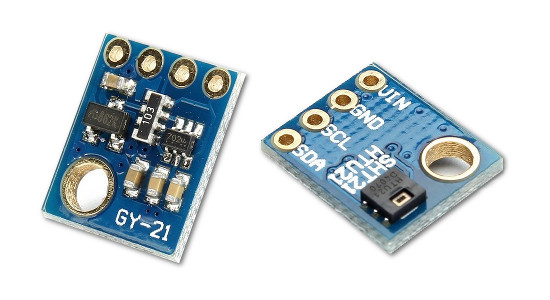
\includegraphics[width=0.4\linewidth]{HTU21.jpg}
	\captionof{figure}{Módulo de Desenvolvimento para o sensor HTU21}
	\label{fig:htu21breakout}
\end{center} 

Possui uma  resolução configurável de 8 bits a 12 bits para a medida de umidade
relativa do ar, que corresponde a 0.7\%RH e 0.04\%RH respectivamente com uma
acurácia de 2\%RH, com duração de conversão é de 3ms (8 bits) a 16ms (12 bits).
O sensor de umidade possui um tempo de resposta de 5 a 10 segundos para uma
excitação em degrau de 33\%RH para 75\%RH. \cite{HTU21DDatasheet}

Já para a medida de temperatura, a resolução é configurável entre 11 bits e 14
bits, representando $0.08\,^{\circ}{\rm C}$ e $0.01\,^{\circ}{\rm C}$
respectivamente, com uma acurácia de $0.3\,^{\circ}{\rm C}$ e com duração da
conversão variando de 7ms (11 bits) a 50ms (14 bits). Possui um tempo de
resposta de 10 segundos para uma excitação em degrau de $15\,^{\circ}{\rm C}$ a
$45\,^{\circ}{\rm C}$.\cite{HTU21DDatasheet}

\subsubsection{Estação de Medidas Bluetooth Low Energy}

A estação de medidas foi projetada para atender os requisitos propostos,
visando o mínimo consumo energético para possibilitar a alimentação através de
baterias sem a necessidade de manutenções frequentes.

Para a transmissão das variáveis medidas pelos sensores utiliza-se o dispositivo
no modo BLE Advertiser, codificando os valores obtidos de forma ordenada dentro
de um pacote de advertising do bluetooth, permitindo que qualquer dispositivo
BLE próximo que seja capaz de detectar a presença da estação de medidas
receba os valores de todas as variáveis medidas.

Este método foi escolhido visando o mínimo consumo de energia por dispensar uma
conexão para a transmissão dos dados.
 
Como diferencial a estação permite a configuração de sua operação através de
serviços GATT do BLE, sendo possível alterar tanto as configurações de rádio
(potêcia e intervalo de transmissão) quanto os parâmetros de configuração dos
sensores (range, escala, intervalo entre medidas). Além disso, os serviços dos
sensores permitem o streaming das novas leituras.

O hardware selecionado para a estação de medidas é o SoC nRF51822, produzido
pela Nordic Semiconductor. Este SoC conta com um processador ARM Cortex M0 de 32
bits e com um transceiver de 2.4GHz multiprotocolo, sendo capaz de operar com
os protocolos Bluetooth e ANT.\cite{nRF51ProdSpec}

A plataforma escolhida leva em consideração as especificações energéticas do
SoC, a possibilidade de depuração do código desenvolvido, a versatilidade de
operar tanto a aplicação quanto o bluetooth dentro do mesmo chip e a
disponibilidade do componente para o uso.

\subsubsubsection{Estratégia para otimização de consumo energético}
Com a finalidade de otimizar o consumo energético foi adotada a estratégia de
manter o microcontrolador em modo deep sleep sempre que possível, sendo o mesmo
acordado somente através de interrupções para a realização das tarefas de rádio
e de leitura de sensores. Durante os períodos em sleep todos os sensores devem
estar num estado de baixo consumo de energia.\cite{MicrochipLPDesign}

Ainda na otimização do consumo, a estratégia adotada para a transmissão dos
dados dos sensores foi concepção do dispositivo operando como um BLE advertiser
pois desta forma se reduz o período no qual há a necessidade do rádio, e
somente durante a configuração o dispositivo opera como um BLE Slave,
permitindo que uma conexão seja estabelecida e que os serviços e
características presentes sejam acessíveis.

\subsubsubsection{Bluetooth Advertiser} 
No modo advertiser, o dispositivo transmite seu endereço MAC e a informação de
que este aceita o estabelecimento de conexões com centrais BLE, que permite
acesso aos serviços BLE que serão descritos posteriormente.
Além disso, estão presentes nos pacotes transmitidos as leituras realizadas
pelos sensores.

As informações dos sensores são codificadas como payload do pacote seguindo a
estrutura de dados no código fonte \ref{lst:struct_adv}. Como formato de
payload, optou-se por utilizar o Manufacturer Specific Data, evitando assim
possíveis conflitos com pacotes BLE definidos pela especificação.

\lstinputlisting[firstline=11,lastline=18,label={lst:struct_adv},
caption={Estrutura de dados para do pacote de leituras dos sensores}]
{../Development/ble-sensor-station/src/libs/ble/advertising/ble_adv_frame.h}

Os pacotes MSD são definidos na especificação suplementar, sendo o data type
definido como  

% -> Utilização do msd
% A transmissão dos pacotes de advertising são feitos através do formato de
% Manufacturer Specific Data, desta garante-se a compatibilidade dos pacotes
% transmitidos por este dispositivo com a especificação sem causar erro
% 
% Codificação do pacote de advertising

\subsubsubsection{Bluetooth Slave}
No modo slave, o dispostivo possui um serviço Bluetooth para cada sensor, com
características que permitem a configuração dos sensores.

O UUID de 128 bits,arbitrariamente utilizado como base para
todos os serviços, está descrito no código fonte \ref{lst:base_uuid}.

\lstinputlisting[firstline=11,lastline=15,label={lst:base_uuid},
caption={Constante que define o UUID base dos serviços Bluetooth}]
{../Development/ble-sensor-station/src/libs/ble/services/ble_services_common.h}

Este UUID foi construído convertendo para hexadecimal o código ASCII da mensagem
\dblquote{UFABCIAR2018\_\_GN}, onde os caracteres \dblquote{\_\_} são os bytes
0x00 deixados em branco para o preenchimento pelo UUID específico dos serviços
bluetooth.

Foram definidos e nomeados quatro serviços Bluetooth para o dispositivo: o APSS
(Air Pressure Sensor Service), o LSS (Luminosity Sensor Service), o THSS
(Temperature and Humidity Sensor Service) e o RPCS (Radio Parameters
Configuration Service).

\newpage
\subparagraph{Air Pressure Sensor Service}(APSS) 
\newline
O APSS é o serviço responsável pela configuração e aquisição de dados do sensor
de pressão BMP180. Este sensor disponibiliza via Bluetooth as informações de
pressão atmosférica e temperatura. Este serviço possui 5 características:
Sensing Interval, Sensor Status, Sensor Resolution, Pressure Data, Temperature
Data.

% \begin{packed_itemize}
%  	\item Sensing Interval
%  	\item Sensor Status
%  	\item Sensor Resolution
%  	\item Pressure Data
%  	\item Temperature Data.
% \end{packed_itemize}

Os identificadores de 2 bytes do serviço e de cada característica estão
definidos no Código Fonte \ref{lst:apss_uuid}. 

\begin{minipage}{0.95\linewidth}
\lstinputlisting[firstline=19,lastline=29,label={lst:apss_uuid},
caption={UUID para o serviço APSS e suas características}]
{../Development/ble-sensor-station/src/libs/ble/services/apss/ble_apss.h}
\end{minipage}

A característica Sensing Interval é uma característica que representa o
intervalo entre as medidas de pressão e temperatura do sensor de BMP180
configurada atualmente. Possui exatamente 4 bytes, o suficiente para armazenar
uma variável do tipo \textbf{uint32\_t}, que representa o intervalo em
milisegundos.

Ao realizar a leitura desta característica, se obtém o intervalo atual entre as
medidas do sensor, e a escrita nesta característica realiza uma nova
configuração. A leitura é permitida sem restrições, já escrita passa pelo
processo de autorização para rejeitar a configuração em caso de valor
inválido. Neste projeto não foi previsto nenhum valor inválido para o intervalo
entre as medidas, porém este recurso possibilita a implementação com menor
retrabalho de software.

A característica Sensor Status indica o estado atual do sensor. Foram previstos
3 estados diferentes para o sensor, como mostra o Código Fonte
\ref{lst:sensor_state_t}. Esta característica possui 1 byte de comprimento, que
pode ser lido a qualquer momento ou escrito com restrições. Os valores aceitos
para a escrita são 0x00 para ligar o sensor e 0x02 para
desligar o sensor.

Os valores definidos são atribuidos pela construção de uma estrutura do tipo
enumeração, sendo o primeiro elemento atribuido com o valor inteiro 0, e
cada novo elemento soma-se 1 unidade ao valor atribuído, conforme
a especificação do enum para a linguagem C.\cite{C99Spec}

\begin{minipage}{0.95\linewidth}
\lstinputlisting[firstline=42,lastline=47,label={lst:sensor_state_t},
caption={Enumeração dos possíveis estados para o sensor}]
{../Development/ble-sensor-station/src/libs/sensing/sensor_public_interface.h}
\end{minipage}

A característica Sensor Resolution determina a resolução e o modo de operação do
sensor. Nesta característica com comprimento de 1 byte, permite-se a leitura sem
restrições e a escrita com validação do valor configurado. Os valores aceitos
para a escrita estão definidos pela enumeração do Código Fonte \ref{lst:bmp180_pwr_mode_t}.
\cite{BMP180Datasheet}

\begin{minipage}{0.95\linewidth}
\lstinputlisting[firstline=14,lastline=21,label={lst:bmp180_pwr_mode_t},
caption={Enumeração dos modos de operação configuráveis para o sensor BMP180s}]
{../Development/ble-sensor-station/src/libs/sensing/bmp180_drv/bmp180_drv.h}
\end{minipage}

As características Pressure Data e Temperature Data são responsáveis pela
transmissão das leituras realizadas pelos sensores. Nelas, armazena-se somente a
leitura mais recente dos sensores sem o acesso ao histórico de leituras. Estas
características permitem apenas a leitura, sem a possibilidade de escrita.
Também está habilitado o recurso de Notify, que permite a transmissão dos
dados lidos dos sensores para o dispositivo conectado sem uma solicação de
leitura, operando num sistema de streaming de dados sempre que uma nova leitura
é realizada.

A característica Pressure Data possui 4 bytes de comprimento, transmitindo os
dados num formato \textbf{uint32\_t}, representando a pressão atmosférica em Pa.
Já a Temperature Data, o comprimento é de 2 bytes, transmitindo a temperatura
num formato \textbf{int16\_t}, sendo que cada unidade representa
$0.01\,^{\circ}{\rm C}$ 

A figura \ref{fig:resumo_apss} representa graficamente a construção do serviço
Air Pressure Sensor Service.

\begin{tcolorbox}[arc=3mm,fontupper=\small,fonttitle=\bfseries,
subtitle style={boxrule=0.4pt, colback=white},colframe=green!25!black,
halign=center,bottom=0mm,
title=Air Pressure Sensor Service]
	\setstretch{1.0}
	UUID de 2 bytes do serviço: 0xABC1h
	
	\begin{tcbitemize}[raster columns=2,raster equal height,fontupper=\footnotesize,
	colbacktitle=yellow!100!red!100!black, coltitle=black,
	fonttitle=\footnotesize\bfseries,size=small, halign=center]
	
	\tcbitem [squeezed title={Sensing Interval Characteristic}]
		\begin{tabular}{ r | l }
		UUID & 0x0A00h \\ \hline
		Tamanho & 4 bytes \\ \hline
		Leitura & Permitida \\ \hline
		Escrita & Permitida com autorização \\ \hline
		Notificação & Desabilitada 
		\end{tabular}

		\tcbitem [squeezed title={Sensor Status Characteristic}]
		\begin{tabular}{ r | l }
		UUID & 0x0A01h \\ \hline
		Tamanho & 1 byte \\ \hline
		Leitura & Permitida \\ \hline
		Escrita & Permitida com autorização \\ \hline
		Notificação & Desabilitada 
		\end{tabular}
		
		\tcbitem [squeezed title={Sensor Resolution Characteristic}]
		\begin{tabular}{ r | l }
		UUID & 0x0A02h \\ \hline
		Tamanho & 1 byte \\ \hline
		Leitura & Permitida \\ \hline
		Escrita & Permitida com autorização \\ \hline
		Notificação & Desabilitada 
		\end{tabular}

		\tcbitem [squeezed title={Pressure Data Characteristic}]
		\begin{tabular}{ r | l }
		UUID & 0x0A03h \\ \hline
		Tamanho & 4 bytes \\ \hline
		Leitura & Permitida \\ \hline
		Escrita & Não permitida \\ \hline
		Notificação & Habilitada 
		\end{tabular}
		
		\tcbitem [squeezed title={Temperature Data Characteristic}]
		\begin{tabular}{ r | l }
		UUID & 0x0A04h \\ \hline
		Tamanho & 2 bytes \\ \hline
		Leitura & Permitida \\ \hline
		Escrita & Não permitida \\ \hline
		Notificação & Habilitada 
		\end{tabular}		
	\end{tcbitemize}
	\tcblower
	\captionof{figure}{Resumo da definição do serviço APSS}\label{fig:resumo_apss}
\end{tcolorbox}

\newpage
\subparagraph{Temperature and Humidity Sensor Service}(THSS) 
\newline

O THSS é o serviço de configuração e aquisição de dados do sensor HTU21D, que
disponibiliza as leituras de temperatura e umidade relativa do ar. O serviço
possui 5 características: Sensing Interval, Sensor Status, Sensor Resolution,
Temperature Data e Humidity Data.

O indentificador de 2 bytes do serviço e de cada característica estão
disponíveis no código fonte \ref{lst:thss_uuid}.

\begin{minipage}{0.95\linewidth}
\lstinputlisting[firstline=22,lastline=28,label={lst:thss_uuid},
caption={UUID para o serviço THSS e suas características}]
{../Development/ble-sensor-station/src/libs/ble/services/thss/ble_thss.h}
\end{minipage}

As características Sensing Interval e Sensor Status seguem as mesmas
especificações do serviço APSS.

A característica Sensor Resolution é uma característica de 1 byte permite a
configuração e leitura da resolução das medidas de temperatura e umidade. As
resoluções das medidas são dependentes uma da outra, sendo as combinações
definidas pelo fabricante. O código fonte \ref{lst:htu21d_resoluion_t} reflete
as opções de resolução oferecidas. Os números indicados na resolução
representam o número de bits.

\begin{minipage}{0.95\linewidth}
\lstinputlisting[firstline=14,lastline=20,label={lst:htu21d_resolution_t},
caption={Enumeração das combinações de resolução do HTU21D}]
{../Development/ble-sensor-station/src/libs/sensing/htu21d_drv/htu21d_drv.h}
\end{minipage}

As características Temperature Data e Humidity Data seguem os mesmos padrões de
apresentação de dados do serviço APSS, sendo possível somente a leitura com
possibilidade de notificação. Ambas possuem o tamanho de 2 bytes, sendo que a
temperatura é transmitida no formato \textbf{int16\_t} enquanto a umidade segue
o formato \textbf{uint16\_t}.

Para a temperatura a unidade transmitida é centésimos de $^{\circ}{\rm C}$,
enquanto a umidade relativa é transmitida em centésimos de \%RH. A conversão de
unidades foi feita para possibilitar a transmissão dos valores com as precisões
lidas pelos sensores sem a necessidade de utilizar ponto flutuante no software e
sem prejuízo aos dados.

A figura \ref{fig:resumo_thss} representa graficamente a construção do serviço
Temperature and Humidity Sensor Service

\begin{tcolorbox}[arc=3mm,fontupper=\small,fonttitle=\bfseries,
subtitle style={boxrule=0.4pt, colback=white},colframe=green!25!black,
halign=center,bottom=0mm,
title=Temperature and Humidity Sensor Service]
	\setstretch{1.0}
	UUID de 2 bytes do serviço: 0xABC2h
	
	\begin{tcbitemize}[raster columns=2,raster equal height,fontupper=\footnotesize,
	colbacktitle=yellow!100!red!100!black, coltitle=black,
	fonttitle=\footnotesize\bfseries,size=small, halign=center]
	
	\tcbitem [squeezed title={Sensing Interval Characteristic}]
		\begin{tabular}{ r | l }
		UUID & 0x0B00h \\ \hline
		Tamanho & 4 bytes \\ \hline
		Leitura & Permitida \\ \hline
		Escrita & Permitida com autorização \\ \hline
		Notificação & Desabilitada 
		\end{tabular}

		\tcbitem [squeezed title={Sensor Status Characteristic}]
		\begin{tabular}{ r | l }
		UUID & 0x0B01h \\ \hline
		Tamanho & 1 byte \\ \hline
		Leitura & Permitida \\ \hline
		Escrita & Permitida com autorização \\ \hline
		Notificação & Desabilitada 
		\end{tabular}
		
		\tcbitem [squeezed title={Sensor Resolution Characteristic}]
		\begin{tabular}{ r | l }
		UUID & 0x0B02h \\ \hline
		Tamanho & 1 byte \\ \hline
		Leitura & Permitida \\ \hline
		Escrita & Permitida com autorização \\ \hline
		Notificação & Desabilitada 
		\end{tabular}

		\tcbitem [squeezed title={Temperature Data Characteristic}]
		\begin{tabular}{ r | l }
		UUID & 0x0B03h \\ \hline
		Tamanho & 2 bytes \\ \hline
		Leitura & Permitida \\ \hline
		Escrita & Não permitida \\ \hline
		Notificação & Habilitada 
		\end{tabular}
		
		\tcbitem [squeezed title={Humidity Data Characteristic}]
		\begin{tabular}{ r | l }
		UUID & 0x0B04h \\ \hline
		Tamanho & 2 bytes \\ \hline
		Leitura & Permitida \\ \hline
		Escrita & Não permitida \\ \hline
		Notificação & Habilitada 
		\end{tabular}		
	\end{tcbitemize}
	\tcblower
	\captionof{figure}{Resumo da definição do serviço THSS}\label{fig:resumo_thss}
\end{tcolorbox}

\newpage
\subparagraph{Luminosity Sensor Service}(LSS) 
\newline
O LSS é o serviço de configuração e aquisição de dados do sensor TSL2561. O
sensor disponibiliza as leituras de luminosidade no espectro visível e
luminosidade no espectro infravermelho. Este serviço possui 6 características:
Sensing Interval; Sensor Status; Integration Time; Sensor Gain; Visible Lux
Data e  Infrared Lux Data.
% \begin{packed_itemize}
%   \item Sensing Interval
%   \item Sensor Status
%   \item Integration Time
%   \item Sensor Gain
%   \item Visible Lux Data
%   \item Infrared Lux Data
% \end{packed_itemize}

Os identificadores de 2 bytes do serviço e de cada característica estão
definidos no Código Fonte \ref{lst:lss_uuid}. 

\begin{minipage}{0.95\linewidth}
\lstinputlisting[firstline=22,lastline=29,label={lst:lss_uuid},
caption={UUID para o serviço LSS e suas características}]
{../Development/ble-sensor-station/src/libs/ble/services/lss/ble_lss.h}
\end{minipage}

As características Sensing Interval e Sensor Status seguem as mesmas
especificações do serviço APSS.

A característica Integration Time configura a janela de amostragem do sensor.
Esta característica permite a leitura do valor atual e permite a escrita com
restrição, já que o sensor possui configurações pré definidas (13.7 ms, 101 ms
ou 402 ms). O Código Fonte \ref{lst:tsl2561_integration_time_t} define os
valores aceitos para escrita nesta característica. \cite{TSL2561Datasheet}

\begin{minipage}{0.95\linewidth}
\lstinputlisting[firstline=14,lastline=19,label={lst:tsl2561_integration_time_t},
caption={Enumeração dos tempos de integração disponíveis para o TSL2561}]
{../Development/ble-sensor-station/src/libs/sensing/tsl2561_drv/tsl2561_drv.h}
\end{minipage}

A característica Sensor Gain permite a configuração e leitura do valor atual do
ganho interno do sensor, que pode ser 0 (sem ganho) ou 16 vezes. A escrita é
permitida com restrição por permitir apenas dois valores. O Código Fonte
\ref{lst:tsl2561_gain_t} define os valores aceitos para escrita nesta
característica.

\begin{minipage}{0.95\linewidth} 
\lstinputlisting[firstline=21,lastline=25,label={lst:tsl2561_gain_t},
caption={Enumeração das opções de ganho para o TSL2561}]
{../Development/ble-sensor-station/src/libs/sensing/tsl2561_drv/tsl2561_drv.h}
\end{minipage}

As características Visible Lux Data e Infrared Lux Data seguem o mesmo padrão
dos outros serviços para a apresentação dos dados, mantendo a última leitura e
com o recurso de Notify habilitado.

Ambas as características possuem 4 bytes de comprimento, transmitindo os dados
num formato \textbf{uint32\_t}, representando as luminosidades correspondentes
em Lux.

A figura \ref{fig:resumo_lss} representa graficamente a construção do serviço
Luminosity Sensor Service.

\begin{tcolorbox}[arc=3mm,fontupper=\small,fonttitle=\bfseries,
subtitle style={boxrule=0.4pt, colback=white},colframe=green!25!black,
halign=center,bottom=0mm,
title=Luminosity Sensor Service]
	\setstretch{1.0}
	UUID de 2 bytes do serviço: 0xABC3h
	
	\begin{tcbitemize}[raster columns=2,raster equal height,fontupper=\footnotesize,
	colbacktitle=yellow!100!red!100!black, coltitle=black,
	fonttitle=\footnotesize\bfseries,size=small, halign=center]
	
	\tcbitem [squeezed title={Sensing Interval Characteristic}]
		\begin{tabular}{ r | l }
		UUID & 0x0C00h \\ \hline
		Tamanho & 4 bytes \\ \hline
		Leitura & Permitida \\ \hline
		Escrita & Permitida com autorização \\ \hline
		Notificação & Desabilitada 
		\end{tabular}

		\tcbitem [squeezed title={Sensor Status Characteristic}]
		\begin{tabular}{ r | l }
		UUID & 0x0C01h \\ \hline
		Tamanho & 1 byte \\ \hline
		Leitura & Permitida \\ \hline
		Escrita & Permitida com autorização \\ \hline
		Notificação & Desabilitada 
		\end{tabular}
		
		\tcbitem [squeezed title={Sensor Integration Time Characteristic}]
		\begin{tabular}{ r | l }
		UUID & 0x0C02h \\ \hline
		Tamanho & 1 byte \\ \hline
		Leitura & Permitida \\ \hline
		Escrita & Permitida com autorização \\ \hline
		Notificação & Desabilitada 
		\end{tabular}
		
		\tcbitem [squeezed title={Sensor Gain Characteristic}]
		\begin{tabular}{ r | l }
		UUID & 0x0C03h \\ \hline
		Tamanho & 1 byte \\ \hline
		Leitura & Permitida \\ \hline
		Escrita & Permitida com autorização \\ \hline
		Notificação & Desabilitada 
		\end{tabular}

		\tcbitem [squeezed title={Pressure Data Characteristic}]
		\begin{tabular}{ r | l }
		UUID & 0x0C04h \\ \hline
		Tamanho & 4 bytes \\ \hline
		Leitura & Permitida \\ \hline
		Escrita & Não permitida \\ \hline
		Notificação & Habilitada 
		\end{tabular}
		
		\tcbitem [squeezed title={Temperature Data Characteristic}]
		\begin{tabular}{ r | l }
		UUID & 0x0C05h \\ \hline
		Tamanho & 4 bytes \\ \hline
		Leitura & Permitida \\ \hline
		Escrita & Não permitida \\ \hline
		Notificação & Habilitada 
		\end{tabular}		
	\end{tcbitemize}
	\tcblower
	\captionof{figure}{Resumo da definição do serviço LSS}\label{fig:resumo_lss}
\end{tcolorbox}

%End of Sensor Station

\subsubsection{Infraestrutura online}

\subsubsubsection{Servidor para recepção}

\subsubsubsection{Armazenamento e Visualização}
%end of infrastructure

\subsubsection{Gateway Bluetooth - Internet}

\subsubsubsection{Especificação}

\subsubsubsection{Bluetooth Observer}

\subsubsubsection{Conectividade}
%end of BLE-Internet gateway
%end of project
\subsection{Implementação}

\subsubsection{Estação de Medidas Bluetooth Low Energy}

% A estação de medidas foi desenvolvida utilizando o SoC NRF51822, produzido pela Nordic
% -> Hardware
% -> Microcontrolador
% -> Sensores		

\subsubsubsection{Ambiente de desenvolvimento}
O ambiente de desenvolvimento foi baseado no Software Development Kit oferecido
pelo fabricante do microcontrolador, o nRF5 SDK 12.3. Este SDK acelera o
desenvolvimento do projeto por diminuir a necessidade de acesso direto aos
registradores do microcontrolador para a operação de hardware, permitindo uma
programação em nível mais elevado.
 
O projeto de firmware foi feito utilizando-se Makefile e o toolchain ARM-GCC,
permitindo assim o desenvolvimento e compilação do projeto de forma
independente de IDE.

A IDE utilizada ao para o desenvolvimento foi o Eclipse IDE versão Oxygen. Além
disso, foram necessárias as ferramentas NRFJPROG, software desenvolvido pelo
fabricante do microcontrolador para realizar tarefas como gravação, leitura,
apagar memória, etc., e a ferramenta Segger J-Link, como interface entre o
computador e o microcontrolador para as operações do NRFJPROG e para a
depuração do firmware.
 
\subsubsubsection{Firmware}

% Estratégia de firmware orientado a eventos
% Linhas gerais sobre firmware para sensores
% Serviços ble
% ADV Encoder/decoder

%End of Sensor Station

\subsubsection{Gateway Bluetooth - Internet}
% 			-> Hardware
% 			-> Ambiente de desenvolvimento
%end of BLE-Internet gateway

\subsubsection{Infraestrutura online}
% -> Ambiente de desenvolvimento	
% -> Coleta e armazenamento de dados
%end of infrastructure
%end of implementation
